\documentclass[11pt, notitlepage]{report}

\usepackage[margin=2cm]{geometry}
\usepackage{amsmath}
\usepackage{graphicx}

\newcommand{\BigO}[1]{\ensuremath{\operatorname{O}\bigl(#1\bigr)}}

\DeclareGraphicsExtensions{.png}

\setlength{\parindent}{0cm}

\title{Randomised Algorithms CW1}
\date{}
\author{Owen Davies \and Charlie Hothersall}

\begin{document}

\maketitle

\section*{Introduction}

In this report we will examine the performance of our implementation of the Skip List, Bloom Filter and Random BInary Search Tree data structures. We will compare the average execution time and the number of comparisons performed for the insert, search and delete operations. The graphs drawn show the performance of the data structures averaged out over 500 repetitions.

\section*{Insertion}

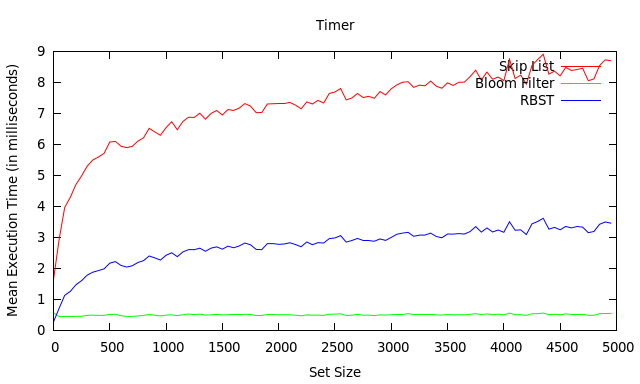
\includegraphics[width=\linewidth]{img/Timer-Add}

Here, the Bloom Filter lives up to it's impressive insertion time of \BigO{k}, with the time being constant (dictated by the 2 hash functions in the implementation) for any set size.\\

The RBST performs very well also, with the mean execution time staying very low even for a large set size. We can see that the line matches a $\log(n)$ graph exactly - our implementation matches the the theoretical prediction of \BigO{\log n} (where n in the set size).\\


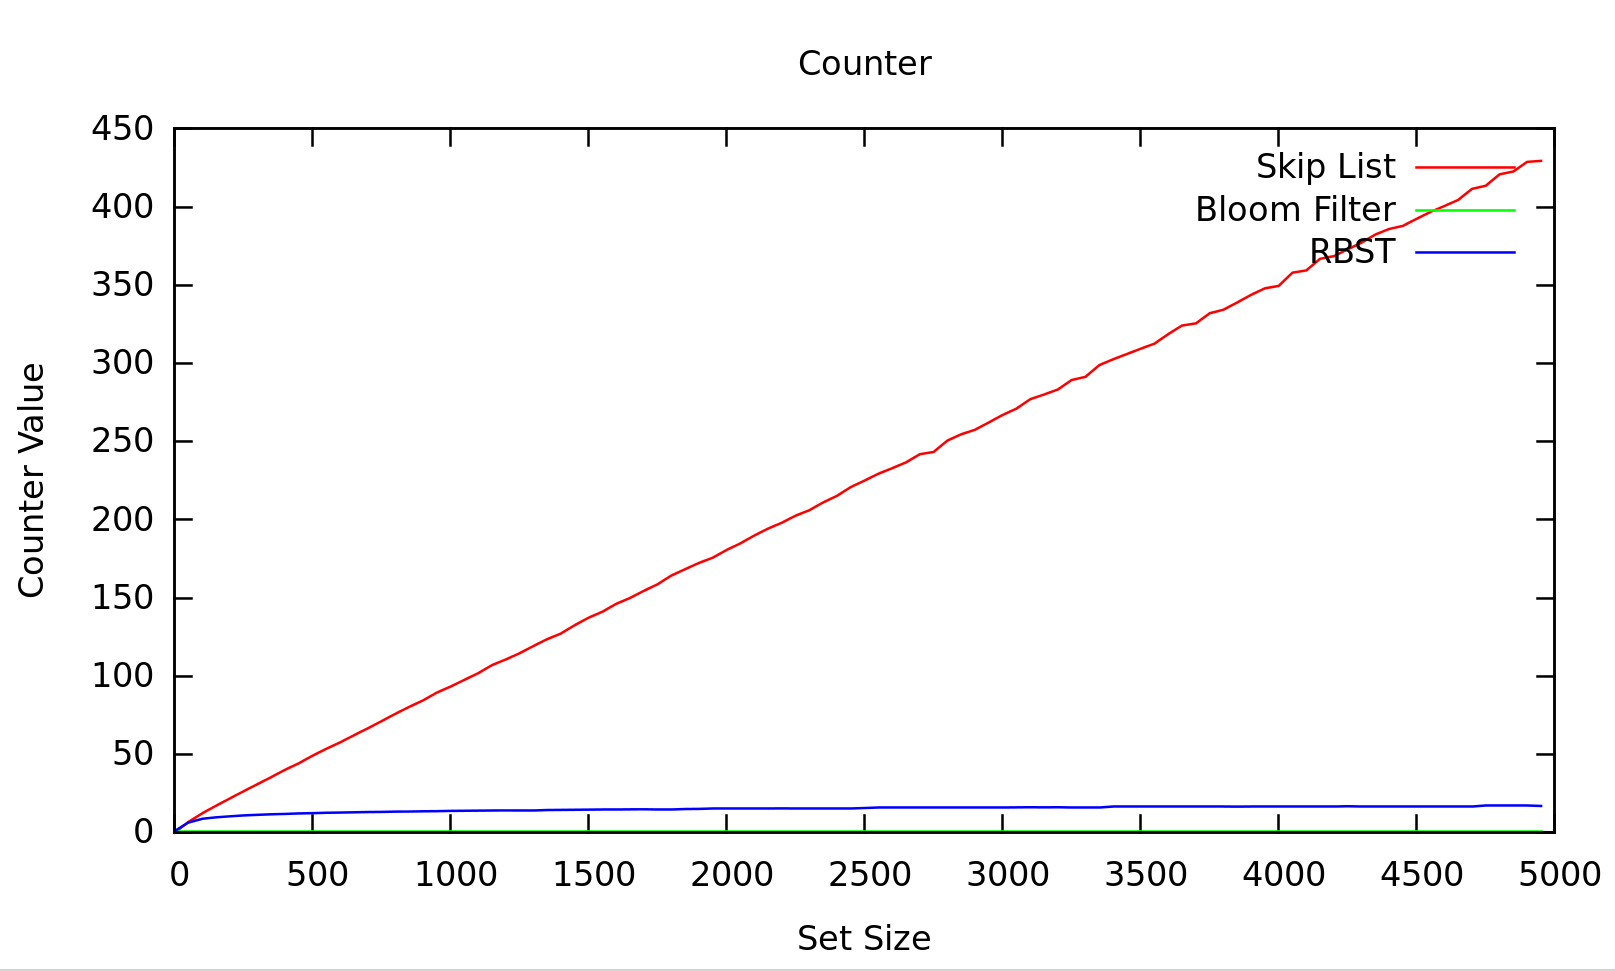
\includegraphics[width=\linewidth]{img/Counter-Add}

The same can be said for the number of comparisons as was said for the execution time. The Bloom Filter is constant for all set sizes as the only computation done is to hash the key and change the correct bits in the filter.\\

The number of comparisons perfomed for RBST insert increases as expected; the bigger the size of the tree, the more recursive calls have to be made. This line still very much conforms to the theoretical complexity of $\log$ n, which makes perfect sense considering the shape of a BST.

\section*{Deletion}

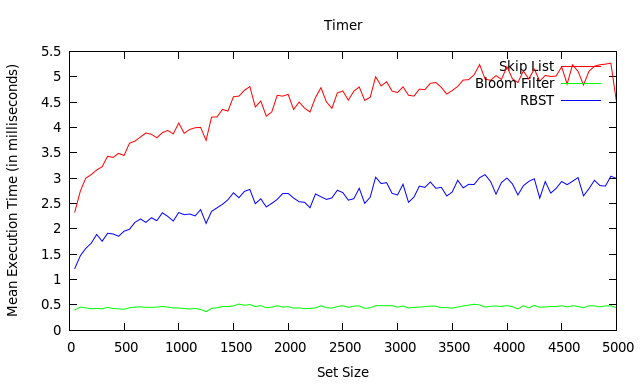
\includegraphics[width=\linewidth]{img/Timer-Del}

As with insertion, the Bloom Filter has a constant time for its violating deletion function, since the delete operation is indentical in terms of computation to the insert operation. The RBST performs at \BigO{\log n} again.

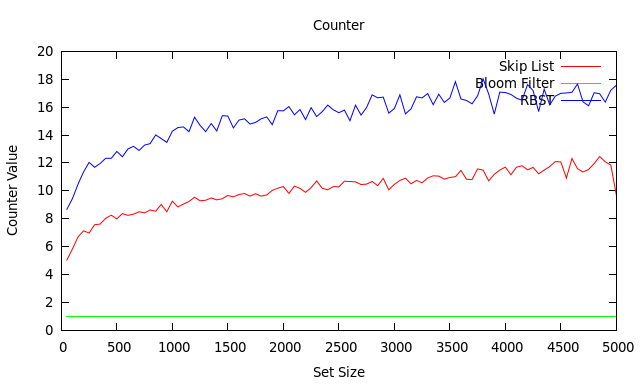
\includegraphics[width=\linewidth]{img/Counter-Del}

The Bloom Filter peforms independantly of set size, with the counter value staying at a constant 1 throughout. The RBST's delete counter value is significantly higher here than it was in the insertion operation. This is somewhat expected since the delete operation is more complex in a binary search tree, and there are a few more cases where recursive calls are made than there are in insertion.\\

This increase means that our implentation does not quite reach the theoretical complexity of \BigO{\log n}, but looking at the graph we can it still follows the shape of a $\log$ n graph, so it appears that the difference is just a small constant value.

\section*{Search}

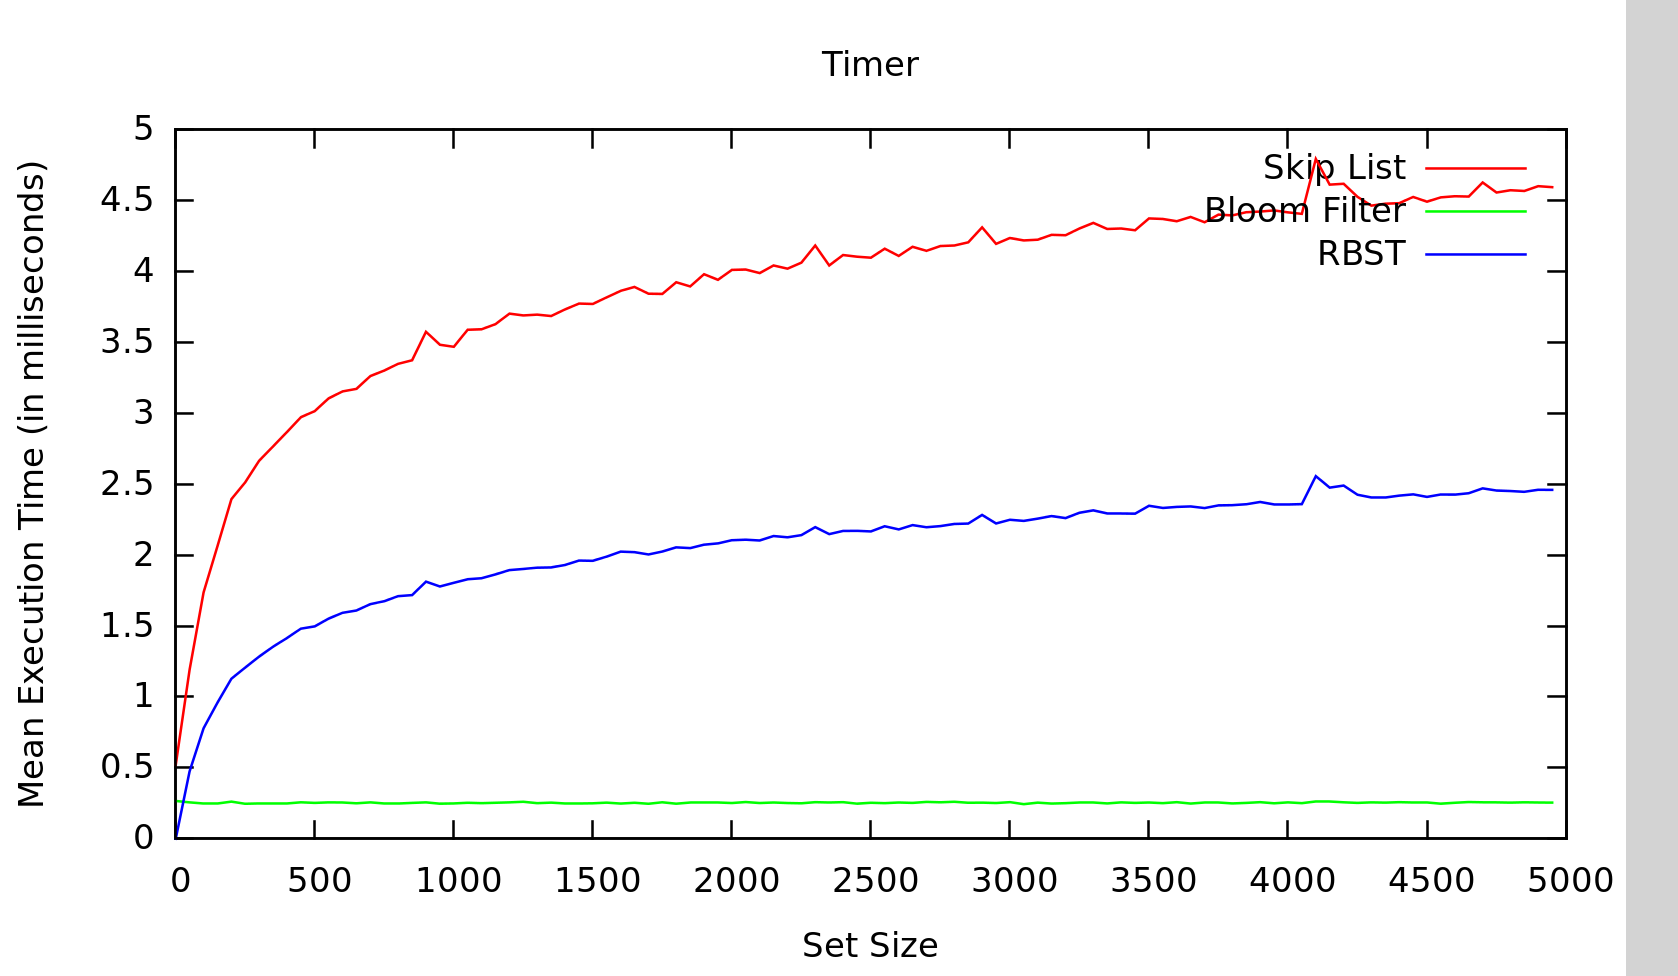
\includegraphics[width=\linewidth]{img/Timer-Find}

As expected, membership test for the Bloom Filter is very fast, and conforms to theoretical \BigO{k} time that we have seen with the toerh operations. Obviously membership test can provide a false positive in the Bloom Filter, but it is clear that if speed is very important then the Bloom Filter is the way to go out of these three structures.\\

Thanks to the randomised nature of the input, the RBST performs well here also. Over a large data set with a lot of repetitions, RBST performs at \BigO{\log_2 n}, as the randomised input ``irons out'' the tree to make it as balanced as possible. This is reflected in the graph above.

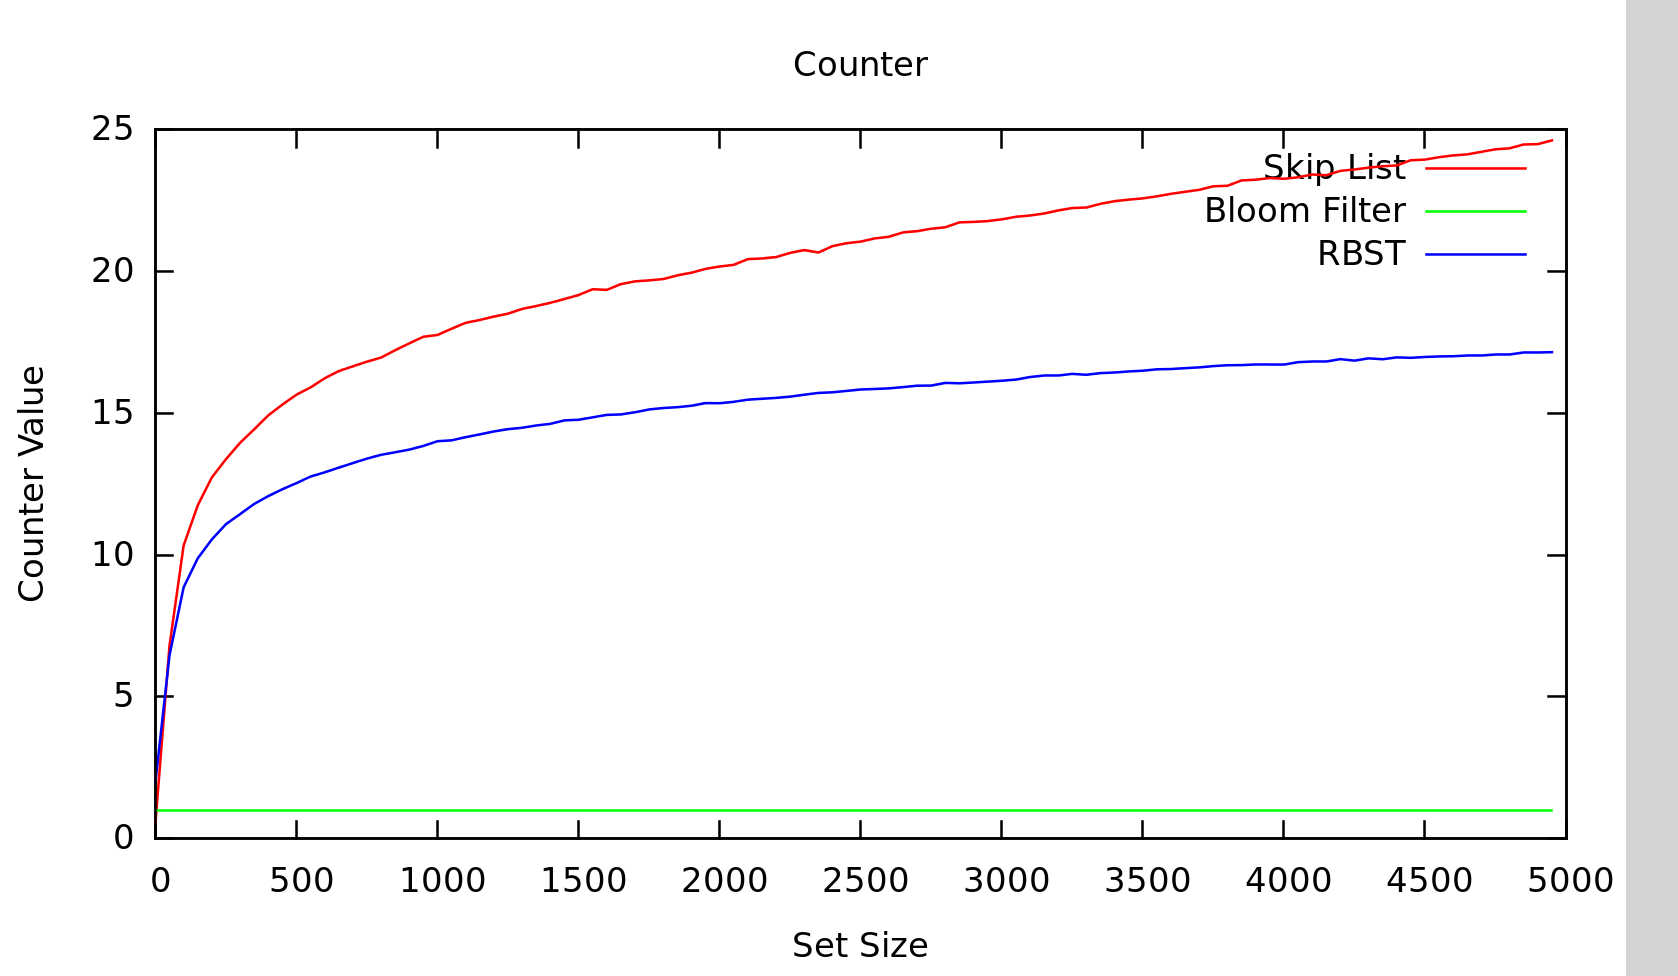
\includegraphics[width=\linewidth]{img/Counter-Find}

The results are fairly standard here. The RBST perfroms at \BigO{\log_2 n} as expected; given that the tree is well balanced there should be $\log_2(n) = h$ recursive calls to the serach function. The Bloom Filter is constant as always.

\end{document}
